\section{Requisitos Técnicos y Operativos}

Aunque los proyectos satelitales suelen definirse por sus prestaciones técnicas, la verdadera viabilidad surge al alinearlas con las restricciones operativas del entorno real. Resulta revelador observar cómo muchos estudios teóricos fallan precisamente al subestimar estas restricciones locales.

\subsection{Requisitos de enlace y QoS}

Uno de los desafíos persistentes al dimensionar enlaces en banda Ka radica en conciliar el apetito de ancho de banda con la degradación atmosférica. Para el VENESAT-2, se establecen umbrales estrictos de desempeño que garanticen servicio confiable incluso bajo condiciones adversas.

Los requisitos mínimos de enlace incluyen un margen de enlace superior a 6 dB para el 99.9\% del tiempo en banda Ku y no inferior a 4.5 dB en Ka para los servicios prioritarios. La calidad de servicio (QoS) exige latencia inferior a 650 ms en modo nominal, BER post-FEC mejor que \(10^{-8}\) y disponibilidad global del sistema superior al 99.95\%. 

Trabajos recientes sobre optimización de enlaces satelitales en frecuencias elevadas resaltan la importancia de técnicas adaptativas como ACM (Adaptive Coding and Modulation) para mantener estos indicadores \cite{LinkBudgetKa2025}. En la práctica, esto implica balances de enlace dinámicos que respondan en tiempo real a variaciones de atenuación.

\begin{table}[h]
\centering
\caption{Requisitos de disponibilidad y desempeño del sistema redundante}
\label{tab:disponibilidad}
\begin{tabular}{lc}
\hline
\textbf{Servicio} & \textbf{Disponibilidad anual requerida} \\
\hline
Televisión y radiodifusión & 99.95\% \\
Internet y datos críticos & 99.90\% \\
Servicios de emergencia & 99.99\% \\
Enlace de respaldo terrestre & 99.80\% \\
Sistema completo (redundante) & >99.95\% \\
\hline
\end{tabular}
\end{table}

La Tabla 3 resume estos umbrales. Particularmente llamativo es el hecho de que los servicios de emergencia exijan niveles cercanos a los estándares militares, lo cual impone arquitecturas robustas desde la fase de diseño.

\subsection{Requisitos operativos y de mantenimiento}

Lejos de ser un detalle secundario, la operatividad diaria define el éxito o fracaso de cualquier sistema satelital en países con limitaciones logísticas. El VENESAT-2 debe contemplar no solo prestaciones en órbita, sino también la capacidad de mantenimiento bajo condiciones venezolanas.

Entre los requisitos operativos destacan: tiempo de conmutación a enlace redundante inferior a 5 segundos, monitoreo 24/7 desde centros de control primario y secundario, y protocolos de mantenimiento preventivo con intervalos compatibles con la disponibilidad de personal técnico calificado. Se exige además compatibilidad con estaciones terrenas existentes y facilidad para actualizaciones remotas de software.

En muchos casos estudiados, la falta de redundancia en el segmento terrestre ha sido causa de interrupciones tan graves como fallos orbitales. Por ello, este estudio prioriza diversidad geográfica entre estaciones principales (por ejemplo, ubicaciones en regiones con diferente régimen pluviométrico) y procedimientos estandarizados de operación.

\subsection{Análisis de riesgos}

Particularmente desafiante resulta anticipar todos los modos de fallo posibles en un sistema tan complejo. La metodología FMEA (Failure Mode and Effects Analysis) ofrece un marco sistemático probado en entornos aeroespaciales para identificar, priorizar y mitigar riesgos críticos.

Aplicando esta aproximación a la arquitectura propuesta del VENESAT-2, se identifican modos de fallo de alta severidad asociados a degradación de amplificadores de potencia en órbita, fallos en los mecanismos de conmutación automática y vulnerabilidades cibernéticas en los enlaces de telemetría y control \cite{FMEASatellite2013}. Cada modo recibe una puntuación RPN (Risk Priority Number) que guía las acciones de mitigación.

\begin{figure}[h]
\centering
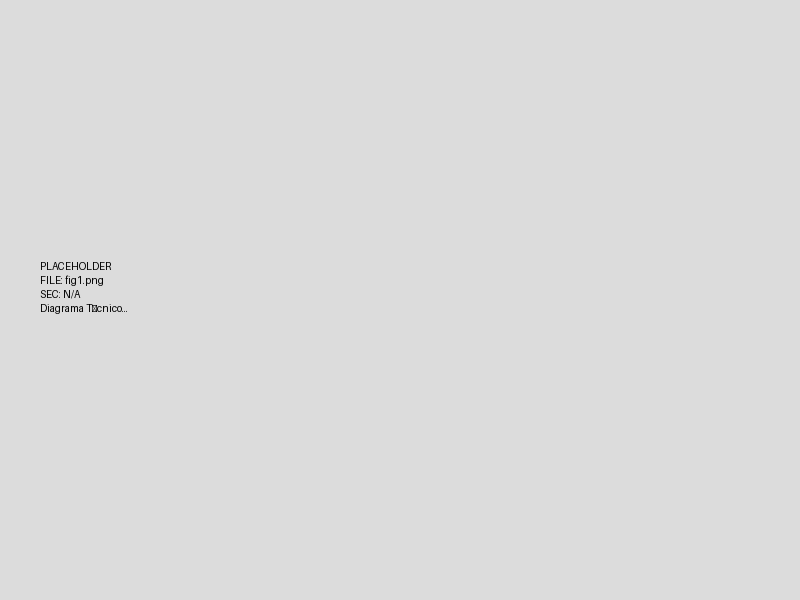
\includegraphics[width=\linewidth]{fig2.png}
\caption{Diagrama de bloques del sistema de enlace satelital redundante propuesto para VENESAT-2}
\label{fig:diagrama_bloques}
\end{figure}

La Figura 2 presenta el diagrama de bloques del sistema, donde se aprecian claramente las rutas principales y redundantes tanto en el segmento espacial como terrestre. Resulta instructivo notar que, aunque la redundancia 1+1 eleva notablemente la confiabilidad, no elimina por completo riesgos correlacionados como tormentas solares o ciberataques dirigidos.

No obstante, cabe matizar que un análisis FMEA exhaustivo, combinado con simulaciones de Monte Carlo, permite reducir sustancialmente la probabilidad de fallos catastróficos. Este enfoque no solo cumple con estándares internacionales, sino que adapta las mejores prácticas a las particularidades operativas y climáticas de Venezuela, sentando bases sólidas para las decisiones de implementación que se discutirán en secciones posteriores.